\section{Experimental Results}

\emph{This section should present your measurements and results--but hold off on the analysis until the next section.  Here we want to \textbf{see} the data you took in the clearest possible way. Go through the Approach you defined in the previous section IN STEPWISE ORDER and record the measurements you've taken in tabular form--referring to the step number for each set of measurements. \textbf{Augment your tables} with charts.  A table is not a substitute for a chart, and a chart is not a substitute for a table.  Each has its purpose.  The chart reveals trends.  The table gives precise numeric values for individual measurements.  Augment your charts with appropriate analysis--ratios, proportions, trends, or other analytics that will help the reader see patterns in your data.}

\emph{It is important to quantify the inherent MEASUREMENT ERROR in any and all measurements you have taken and to give the basis for the error. Have you quantified the errors in your measurement?  All measurements are imprecise.  Estimate your measurement error, and explain the sources of error.  Represent the error ranges with error bars in your charts.  See the example below.}

We present the averaged results, over 10 runs, in Table~\ref{table:summarytable}, which were taken in Step 5 of our experiment.

\begin{figure}[h]
\centering
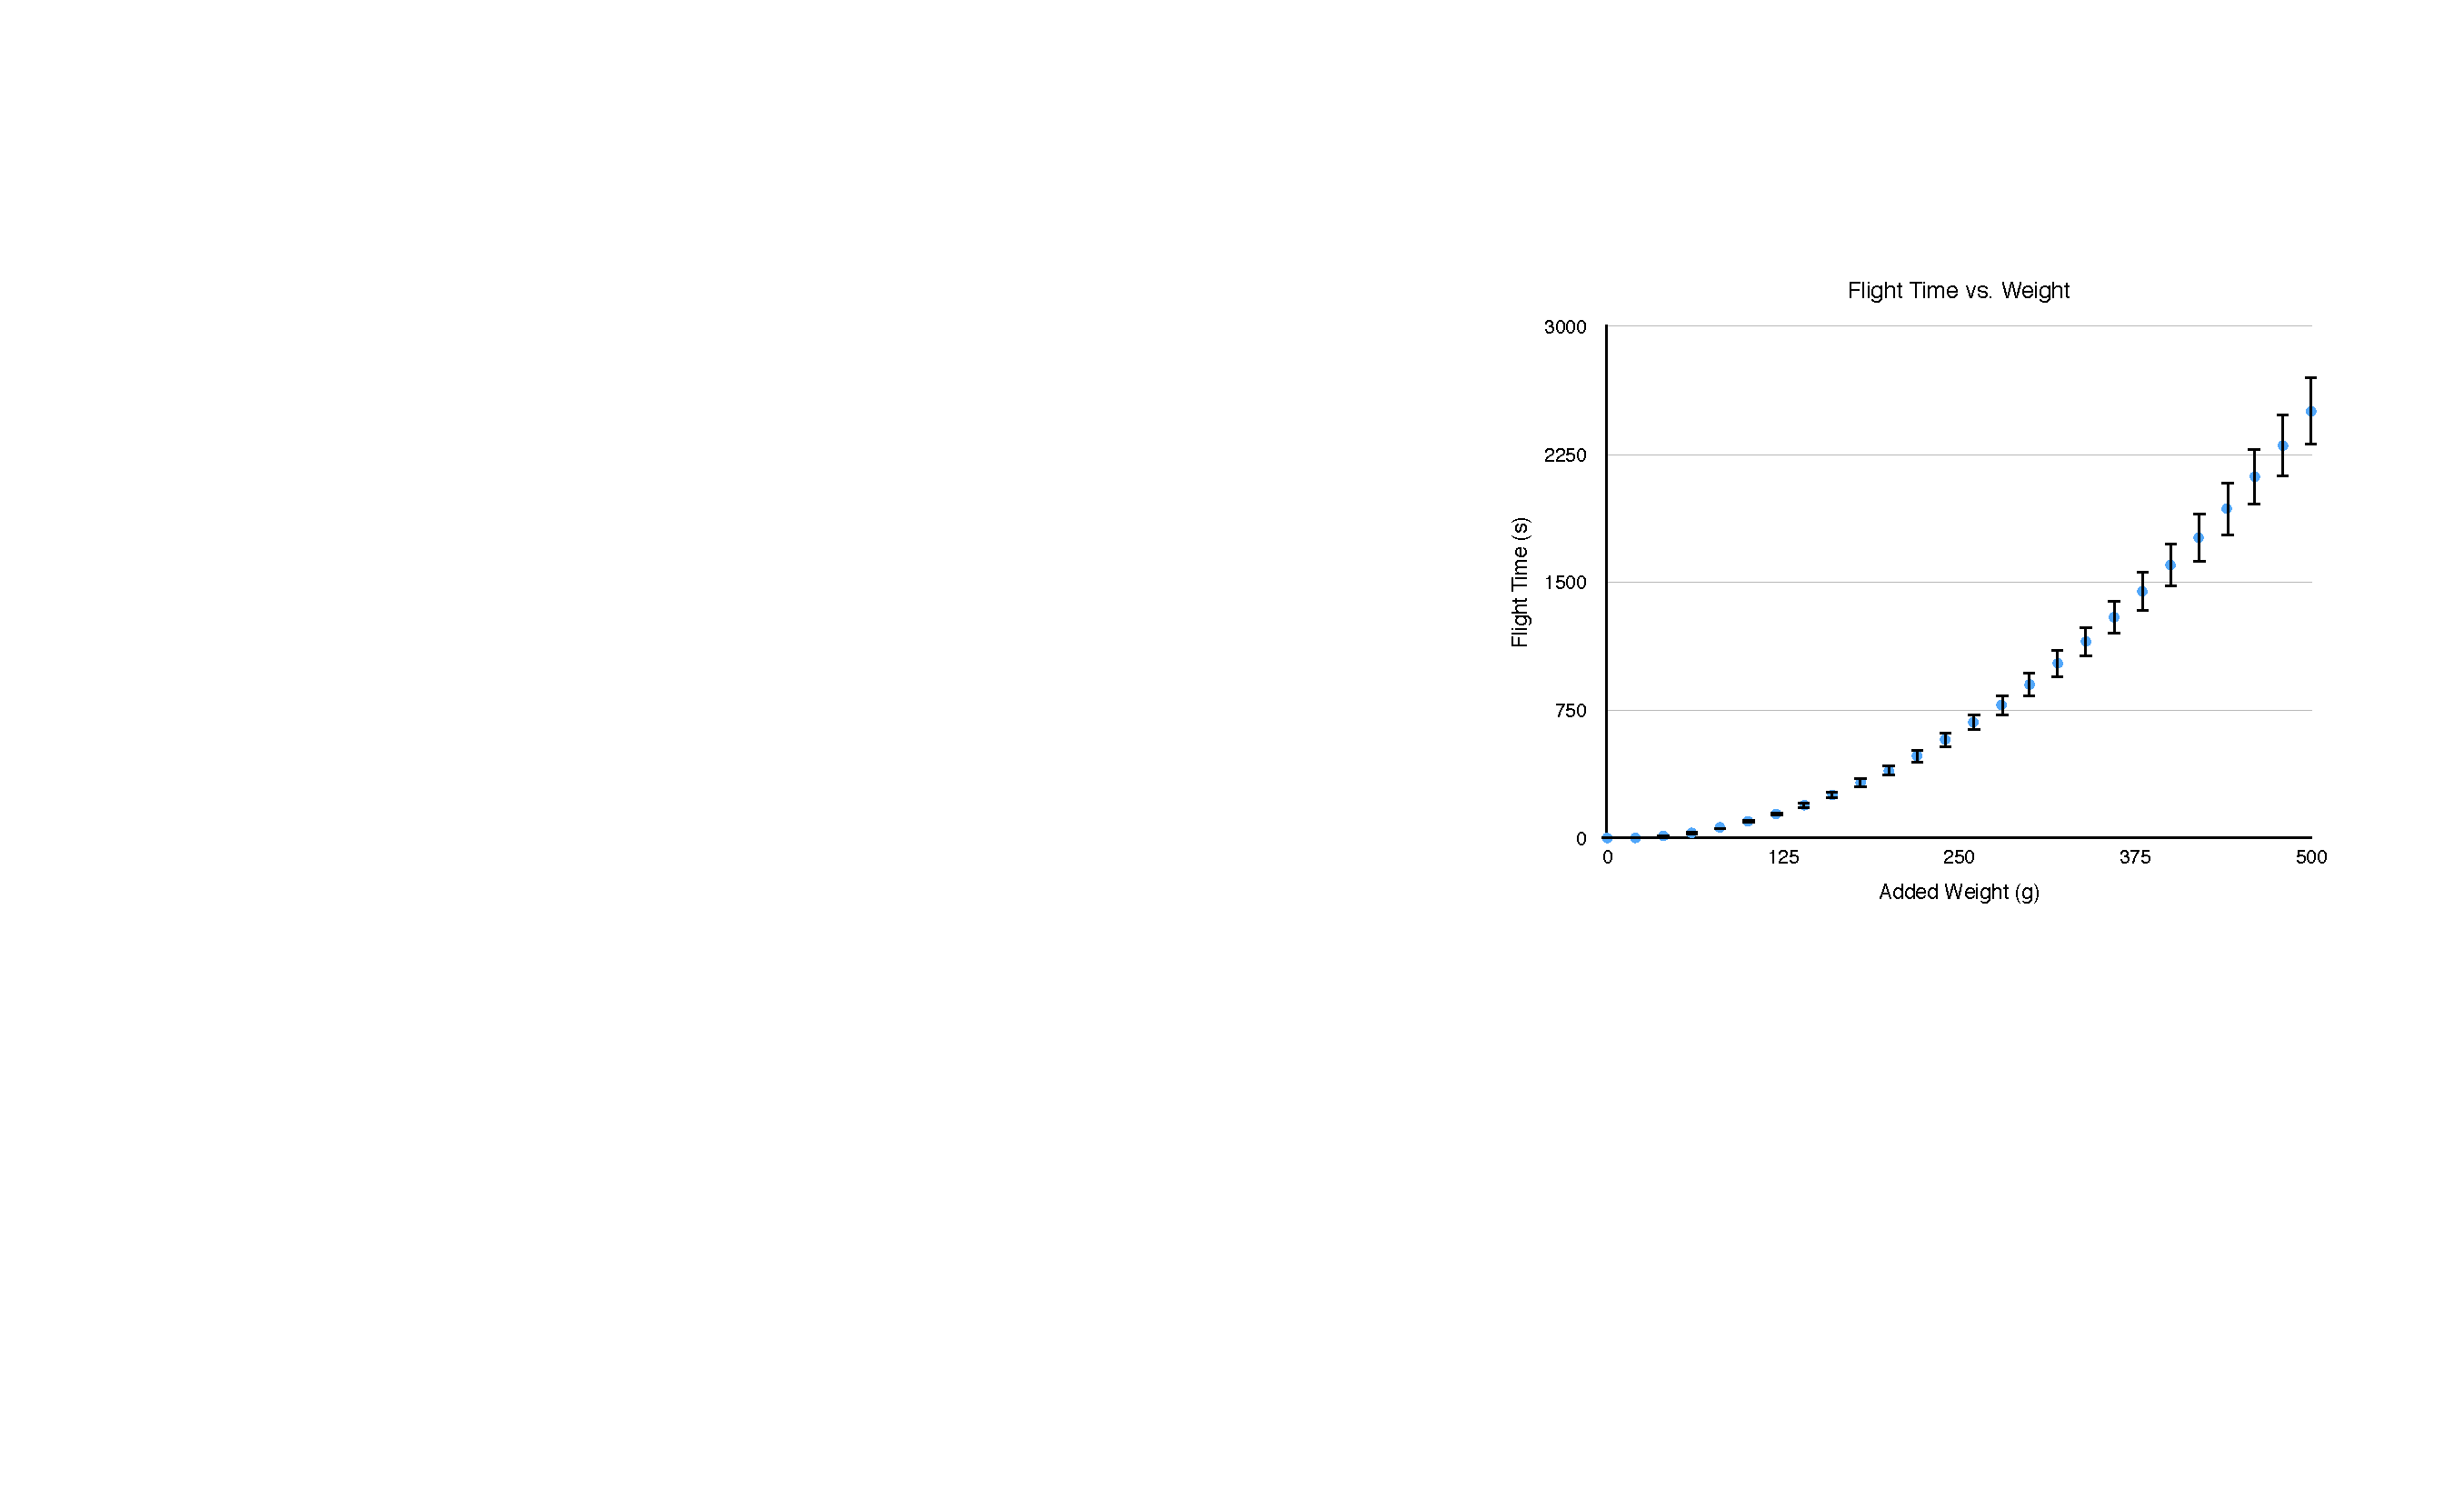
\includegraphics[width=0.4\textwidth]{chart}
\caption{Flight time vs. weight, averaged over 10 runs.}
\label{fig:chart}
\end{figure}

Figure~\ref{fig:chart} shows this data plotted on a chart. In this case, the error bars represent the standard deviation of the results from the 10 runs.

\begin{table}[t]
\caption{Summary of results}
\label{table:summarytable}
\begin{center}
\begin{tabular}{cc}
\bf Added Weight (g) & \bf Flight Time (s)
\\ \hline \\
0 & 2.05  \\
100 &100.1 \\
200 &395.4 \\
300 & 902.1 \\
400 & 1601.8 \\
500 & 2502.8 \\

\end{tabular}
\end{center}
\end{table}

We report flight time here, but we should also have reported and graphed air-speed ($\frac{distance}{flight-time}$) as a function of weight.

Note that we observed \textbf{no statistically significant variation} in performance between the African and the European swallows.  We should have plotted a correlelogram, but we didn't.
